
% !TEX TS-program = pdflatex
\documentclass[11pt]{article}

\usepackage[margin=1in]{geometry}
\usepackage{amsmath, amssymb, amsthm}
\usepackage{mathtools}
\usepackage{hyperref}
\usepackage{enumitem}
\usepackage{listings}
\usepackage{xcolor}
\usepackage{tikz}
\usetikzlibrary{arrows.meta, positioning, shapes.geometric}

\hypersetup{
  colorlinks=true,
  linkcolor=blue,
  urlcolor=blue,
  citecolor=blue
}

\newtheorem{theorem}{Theorem}[section]
\newtheorem{lemma}[theorem]{Lemma}
\newtheorem{proposition}[theorem]{Proposition}
\newtheorem{corollary}[theorem]{Corollary}
\theoremstyle{definition}
\newtheorem{definition}[theorem]{Definition}
\newtheorem{remark}[theorem]{Remark}
\newtheorem{example}[theorem]{Example}
\newtheorem{openproblem}[theorem]{Open Problem}

\newcommand{\Fin}{\mathrm{Fin}}
\newcommand{\NN}{\mathbb{N}}
\newcommand{\RR}{\mathbb{R}}
\newcommand{\EE}{\mathbb{E}}
\newcommand{\Prob}{\mathbb{P}}
\newcommand{\lean}[1]{\texttt{#1}}

\definecolor{leanblue}{RGB}{40, 80, 140}
\definecolor{leanbg}{RGB}{248, 248, 252}
\definecolor{gapred}{RGB}{180, 40, 40}
\definecolor{provedgreen}{RGB}{30, 120, 50}

\lstdefinelanguage{lean4}{
  morekeywords={def, theorem, lemma, structure, abbrev, namespace, open,
    noncomputable, section, variable, where, instance, class,
    import, set_option, deriving, attribute, scoped,
    by, intro, rcases, exact, refine, have, let, letI, set, calc, simp,
    match, with, if, then, else, return, do,
    Prop, Type, Sort, Nat, Bool, List, Fin, Set, Measure, ENNReal},
  sensitive=true,
  morecomment=[l]{--},
  morecomment=[n]{/-}{-/},
  morestring=[b]",
  literate={→}{{$\to$}}1 {←}{{$\leftarrow$}}1 {∀}{{$\forall$}}1 {∃}{{$\exists$}}1
    {∧}{{$\wedge$}}1 {∨}{{$\vee$}}1 {¬}{{$\lnot$}}1 {≤}{{$\le$}}1 {≥}{{$\ge$}}1
    {≠}{{$\ne$}}1 {⊆}{{$\subseteq$}}1 {∈}{{$\in$}}1 {∉}{{$\notin$}}1
    {×}{{$\times$}}1 {⟨}{{$\langle$}}1 {⟩}{{$\rangle$}}1
    {ℕ}{{$\mathbb{N}$}}1 {ℝ}{{$\mathbb{R}$}}1
    {∂}{{$\partial$}}1 {∫⁻}{{$\int^-$}}2
    {₀}{{$_0$}}1 {₁}{{$_1$}}1 {₂}{{$_2$}}1
    {α}{{$\alpha$}}1 {β}{{$\beta$}}1 {θ}{{$\theta$}}1 {μ}{{$\mu$}}1
    {π}{{$\pi$}}1 {ω}{{$\omega$}}1 {σ}{{$\sigma$}}1 {τ}{{$\tau$}}1
    {⁺}{{$^+$}}1 {⁻}{{$^-$}}1
    {:=}{{$\coloneqq$}}2,
}

\lstset{
  language=lean4,
  basicstyle=\ttfamily\small,
  keywordstyle=\color{leanblue}\bfseries,
  commentstyle=\itshape\color{gray},
  backgroundcolor=\color{leanbg},
  frame=single,
  framerule=0.4pt,
  rulecolor=\color{gray!50},
  breaklines=true,
  columns=flexible,
  xleftmargin=1em,
  framexleftmargin=0.5em,
  aboveskip=0.8em,
  belowskip=0.8em,
}

\title{Formalizing the Markov de Finetti Theorem in Lean~4:\\
  Current Status and Open Gap\\[0.3em]
  {\large Mettapedia project technical note}}
\author{}
\date{April 2026}

\begin{document}
\maketitle

\begin{abstract}
We report on an ongoing Lean~4 formalization of the Markov de Finetti theorem
(Diaconis--Freedman 1980): every Markov-exchangeable, recurrent prefix measure
on a finite alphabet is a mixture of time-homogeneous Markov chains.

The formalization is a partial success with a precisely characterized gap.
The \emph{internal} representation theorem---given an extension to infinite
trajectories together with explicit row-kernel data, construct the mixing
measure---is fully proved (zero \texttt{sorry}).  The carrier transport
bijection---an evidence-preserving Equiv between finite prefix carriers
for adjacent visit indices---is fully proved (1465 lines, zero \texttt{sorry}).
The \emph{literature-facing} theorem, which derives the row-kernel data
from bare Markov exchangeability and recurrence, requires a bridge from
the proved carrier transport to the proved de Finetti infrastructure.

A structural audit (April 2026) identified three bugs in the gap
characterization: (1) the evidence-preserving Equiv is used far below
its full strength (only 1D marginals extracted when it preserves all
transition counts); (2) the zero-sorry count masks unproved mathematical
content encoded as assumption interfaces; (3) an archived Euler trail
infrastructure (1225 lines, 0 sorry) provides a more direct route to
the missing bridge.  The corrected proof strategy (\S\ref{sec:strategy})
estimates $\sim$530 lines of new code to close the gap entirely,
primarily a bridge from evidence preservation to successor-matrix
partial exchangeability.

The formalization comprises approximately 50{,}000 lines of Lean across
12 active files, with an additional 43{,}000 lines formalizing the classical
(i.i.d.) de Finetti theorem via three independent proof strategies.
All active code compiles with zero \texttt{sorry}.
\end{abstract}

\tableofcontents

%% ========================================================================
\section{Introduction and Motivation}
%% ========================================================================

Solomonoff induction (1964) provides a universal Bayesian mixture over all
computable hypotheses.  In practice, one restricts to structured hypothesis
classes---i.i.d.\ models, finite-state Markov models, hidden Markov models---for
tractability and interpretability.  The conceptual bridge is:

\begin{quote}
\emph{Exchangeability (or partial exchangeability) assumptions identify when a
rich family of distributions can be represented as a mixture over a simpler
parametric family.}
\end{quote}

For i.i.d.\ sequences, de Finetti's theorem (1931/1937) gives
$\text{exchangeability} \Rightarrow \text{mixture of i.i.d.\ laws}$.
For Markov sequences, Diaconis and Freedman (1980) show a corresponding
representation for \emph{Markov-exchangeability}, with an additional
\emph{recurrence} hypothesis.

Once such structure theorems are formalized, they justify \emph{structured
universal mixtures}: Solomonoff-like prediction instantiated by mixing over
the parametric space of Markov models, with hyperpriors retaining
dominance-style guarantees.  This is the broader program that motivates the
formalization.

\paragraph{Status summary.}
The internal representation theorem is proved: given an extension measure $P$
on infinite trajectories together with explicit row-kernel crux data, we
construct the mixing measure $\pi$ on the Markov parameter space and verify
$\mu(xs) = \int \mathrm{wordProb}_\theta(xs)\, d\pi(\theta)$ for all finite
words $xs$.

The literature-facing theorem---deriving the row-kernel data from bare
Markov exchangeability and recurrence---requires three sub-obligations
(Section~\ref{sec:gap}) that remain open.  A structural audit
(\S\ref{sec:crossrow}) identified a previously overlooked gap in the
cross-row coherence argument.

%% ========================================================================
\section{Mathematical Setup}
\label{sec:setup}
%% ========================================================================

Throughout, $k \ge 1$ is a fixed positive integer and the state space is
$A = \Fin(k)$.

\subsection{Prefix measures}

A \emph{prefix measure} assigns a nonneg\-ative extended real to each finite
word over $A$, satisfying cylinder consistency:
$\mu(\varepsilon) = 1$ and $\mu(xs) = \sum_{a \in A} \mu(xs \cdot [a])$.
In the Lean development, this is modeled as:
\begin{lstlisting}
-- FiniteAlphabet.PrefixMeasure (Fin k)
-- A function List (Fin k) → ENNReal satisfying consistency
\end{lstlisting}

\subsection{Transition counts and Markov evidence}

For a trajectory $x_0, x_1, \ldots, x_n$ over $\Fin(k)$, the Markov
sufficient statistics are the starting state $x_0$ and the transition-count
matrix $N(i,j) = \#\{t < n : x_t = i,\; x_{t+1} = j\}$.

\begin{lstlisting}
def transCount (xs : Fin (n + 1) → α) (a b : α) : ℕ :=
  (univ.filter (fun i : Fin n =>
    xs (Fin.castSucc i) = a ∧ xs (Fin.succ i) = b)).card

structure MarkovEvidence (α : Type*) where
  start : α
  trans : α → α → ℕ

def evidenceOf (xs : Fin (n + 1) → α) : MarkovEvidence α :=
  { start := xs 0
    trans := fun a b => transCount xs a b }
\end{lstlisting}

\subsection{Markov exchangeability}

A prefix measure is \emph{Markov-exchangeable} when $\mu(xs)$ depends only
on the Markov evidence, not on the detailed order of transitions:

\begin{lstlisting}
def FiniteMarkovExchangeable (n : ℕ)
    (X : Fin (n + 1) → Ω → α) (μ : Measure Ω) : Prop :=
  ∀ vals₁ vals₂ : Fin (n + 1) → α,
    evidenceOf vals₁ = evidenceOf vals₂ →
      μ (cylinder X vals₁) = μ (cylinder X vals₂)
\end{lstlisting}

For prefix measures (rather than random variables), the corresponding
predicate is:

\begin{lstlisting}
def MarkovExchangeablePrefixMeasure
    (μ : PrefixMeasure (Fin k)) : Prop :=
  ∀ xs ys : List (Fin k),
    -- if xs and ys have the same length and same evidence:
    (∃ (n : ℕ), xs = List.ofFn xs_fin ∧
      ys = List.ofFn ys_fin ∧
      evidenceOf xs_fin = evidenceOf ys_fin) →
      μ xs = μ ys
\end{lstlisting}

\begin{example}[Worked example: $k=2$, trajectory of length 4]
\label{ex:worked}
Let $A = \{0, 1\}$ and consider the trajectory $xs = [0, 1, 0, 1]$ of
length 4 (so $n = 3$).  The Markov evidence is:
\[
\mathrm{start} = 0, \qquad
N = \begin{pmatrix} 0 & 2 \\ 1 & 0 \end{pmatrix},
\]
recording two $0 \to 1$ transitions and one $1 \to 0$ transition.
The trajectory $[0, 1, 1, 0]$ has evidence
$\mathrm{start} = 0$,
$N = \bigl(\begin{smallmatrix} 0 & 1 \\ 1 & 1 \end{smallmatrix}\bigr)$,
which differs (one fewer $0 \to 1$, one more $1 \to 1$).
A Markov-exchangeable measure may assign different probabilities to these.

However, $[0, 1, 0, 1]$ and any other length-4 trajectory starting at $0$
with the same count matrix $N$ must receive the same probability.  In this
case, no other trajectory has exactly this count matrix, so the equivalence
class is a singleton.

The parameter space $\Theta_2 = \mathrm{MarkovParam}(2)$ is
$\Delta_1 \times \Delta_1 \times \Delta_1$: an initial distribution on
$\{0,1\}$ (a single parameter $p_0 = \Prob(X_0 = 0)$), and two
row-stochastic transition probabilities $p_{0 \to 1}$ and $p_{1 \to 0}$.
For $\theta = (p_0, p_{0\to1}, p_{1\to0})$:
\[
\mathrm{wordProb}_\theta([0,1,0,1])
= p_0 \cdot p_{0\to1} \cdot p_{1\to0} \cdot p_{0\to1}
= p_0 \cdot p_{0\to1}^2 \cdot p_{1\to0}.
\]
The representation theorem, when applicable, gives
$\mu([0,1,0,1]) = \int_{\Theta_2} p_0 \cdot p_{0\to1}^2 \cdot p_{1\to0}\, d\pi(\theta)$
for some probability measure $\pi$ on $\Theta_2$.
\end{example}

\subsection{Markov parameter space and word probability}

A Markov model on $\Fin(k)$ is parameterized by an initial distribution
$\pi_0$ and a row-stochastic transition kernel $P(i,\cdot)$:

\[
\mathrm{wordProb}_\theta(x_0, \ldots, x_n)
\;=\; \pi_0(x_0) \cdot \prod_{t=0}^{n-1} P(x_t, x_{t+1}).
\]

The parameter space $\Theta_k = \mathrm{MarkovParam}(k)$ is a finite product
of simplices, hence compact.  The function
$\theta \mapsto \mathrm{wordProb}_\theta(xs)$ is continuous on $\Theta_k$.

\subsection{Recurrence}

Markov exchangeability alone does \emph{not} imply a mixture representation.
A counterexample is constructed in the Lean development: consider $k = 2$
with the deterministic chain $0 \to 1 \to 1 \to 1 \to \cdots$ (the chain
leaves state~0 at step~1 and never returns).  This prefix measure is
Markov-exchangeable---the only trajectory of any given length starting at~0
is the all-ones tail, so the ``permutation'' equivalence class is always
a singleton, and the condition holds vacuously.  But it cannot be
represented as a mixture of time-homogeneous Markov chains, because any
non-degenerate mixture would assign positive probability to trajectories
that return to~0, contradicting the deterministic behavior.

The Diaconis--Freedman recurrence condition requires the trajectory to
return to its starting state infinitely often, almost surely:

\begin{lstlisting}
def recurrentEvent : Set (ℕ → Fin k) :=
  ⋂ N : ℕ, ⋃ n ≥ N, returnEvent n

def MarkovRecurrentPrefixMeasure
    (μ : PrefixMeasure (Fin k)) : Prop :=
  ∃ (P : Measure (ℕ → Fin k)),
    IsProbabilityMeasure P ∧
    (∀ xs : List (Fin k),
      μ xs = P (cylinder xs)) ∧
    P (recurrentEvent) = 1
\end{lstlisting}

Recurrence is an \emph{identifiability anchor}: it guarantees the trajectory
keeps resampling transitions, allowing long-run statistics to stabilize.

%% ========================================================================
\section{What Is Proved}
\label{sec:proved}
%% ========================================================================

All results in this section compile with zero \texttt{sorry} in Lean~4
with Mathlib.

\subsection{Dirichlet conjugacy and structured predictors}

The Dirichlet-multinomial conjugate prior pattern is formalized for
$k$-ary alphabets.  Evidence is a vector of counts:

\begin{lstlisting}
structure MultiEvidence (k : ℕ) where
  counts : Fin k → ℕ

structure DirichletParams (k : ℕ) where
  priorParams : Fin k → ℝ
  params_pos : ∀ i, 0 < priorParams i
\end{lstlisting}

The key theorem states that Bayesian update equals coordinatewise count
addition---the conjugacy that makes finite-dimensional Markov inference
tractable:

\begin{lstlisting}
-- Verbatim from EvidenceDirichlet.lean:
theorem evidence_aggregation_is_dirichlet_update
    (prior : DirichletParams k)
    (e₁ e₂ : MultiEvidence k) (i : Fin k) :
    (⟨prior, e₁ + e₂⟩ :
      EvidenceDirichletParams k).posteriorParam i =
    (⟨prior, e₁⟩ :
      EvidenceDirichletParams k).posteriorParam i
    + e₂.counts i
\end{lstlisting}

Here \lean{EvidenceDirichletParams} bundles a prior with observed evidence,
and \lean{posteriorParam i} returns $\alpha_i + n_i$ (the $i$-th Dirichlet
posterior parameter).  The theorem says combining evidence and then computing
the posterior is the same as computing the posterior of the first batch and
adding the second batch's counts---the Dirichlet conjugate update pattern.

Building on this, a finite-alphabet Markov(1) predictor with one
Dirichlet prior per transition row is constructed
(\lean{MarkovDirichletPredictor.lean}, 497 lines).

A \emph{universal hyperprior mixture} over a countable family of symmetric
Dirichlet priors (parameter $a \in \{1/2, 1, 3/2, \ldots\}$, including the
Jeffreys and Laplace choices) is then constructed with computable weights
and dominance guarantees
(\lean{MarkovDirichletHyperpriorMixture.lean}).

\subsection{Domain restriction: Markov exchangeability implies count sufficiency}

The bridge file (\lean{MarkovExchangeabilityBridge.lean}, 600+ lines)
establishes that Markov exchangeability of a prefix measure implies
predictions factor through transition-count evidence.  The key
constructions are:

\begin{lstlisting}
-- Extract the transition-count summary from a trajectory:
def countsOfFn (xs : Fin (n + 1) → Fin k) :
    TransCounts k :=
  ⟨fun a b => transCount xs a b⟩

-- Verify the summary agrees with the evidence:
theorem summary_ofFn (xs : Fin (n + 1) → Fin k) :
    TransCounts.summary (List.ofFn xs) =
      some (countsOfFn xs, xs (Fin.last n))
\end{lstlisting}

This is the Markov analogue of the i.i.d.\ count-sufficiency result:
under Markov exchangeability, two trajectories with the same start state
and transition counts receive the same probability, regardless of
the order in which transitions occur.

\subsection{Visit-time infrastructure (hard direction)}

The hard direction of the Markov de Finetti theorem requires decomposing
trajectories by \emph{visit times} to each state.  The Core file
(\lean{MarkovDeFinettiFortiniBridgeCore.lean}, 1843 lines) formalizes:

\begin{lstlisting}
def visitCountBefore (ω : ℕ → Fin k) (i : Fin k)
    (t : ℕ) : ℕ :=
  Finset.sum (Finset.range t)
    (fun s => if ω s = i then 1 else 0)

def isNthVisitTime (ω : ℕ → Fin k) (i : Fin k)
    (n t : ℕ) : Prop :=
  ω t = i ∧ visitCountBefore ω i t = n

noncomputable def rowSuccessorAtNthVisit
    (i : Fin k) (n : ℕ) (ω : ℕ → Fin k) : Fin k :=
  match nthVisitTime ω i n with
  | some t => successorAt ω t
  | none => i
\end{lstlisting}

For each state $i$, the \emph{row-successor process}
$n \mapsto \mathrm{rowSuccessorAtNthVisit}(i, n, \omega)$
records the state visited \emph{after} the $n$-th visit to $i$.
Under Markov exchangeability, this process has strong symmetry properties.

\subsection{The internal representation theorem}
\label{sec:internal}

The central achievement of the formalization is the \emph{internal}
representation theorem.  It requires as input:

\begin{enumerate}[leftmargin=2em]
\item An extension $P$ (a probability measure on $\NN \to \Fin(k)$)
  whose cylinders agree with $\mu$.
\item A family of row kernels
  $\mathrm{rowKernel} : \Fin(k) \to (\NN \to \Fin(k)) \to
  \mathrm{ProbabilityMeasure}(\Fin(k))$.
\item \emph{Row-kernel crux data}: measurability conditions, start-restricted
  invariance, and a cross-row coherence step.
\end{enumerate}

\begin{definition}[Cross-Anchor Product Identity]
The cross-anchor product identity asserts that cylinder probabilities under
$P$ decompose as integrals of row-kernel step products, conditioned on
the starting state:
\begin{lstlisting}
def CrossAnchorProductIdentity
    (P : Measure (ℕ → Fin k))
    (rowKernel : Fin k → (ℕ → Fin k)
      → ProbabilityMeasure (Fin k)) : Prop :=
  ∀ (a b : Fin k) (xs : List (Fin k)),
    P (cylinder (a :: b :: xs)) =
      ∫⁻ ω, (if ω 0 = a
        then rowKernelStepProd rowKernel ω
               (a :: b :: xs)
        else 0) ∂P
\end{lstlisting}
\end{definition}

\begin{definition}[Row-Kernel Crux Data]
\label{def:cruxdata}
The crux data bundles four conditions on a row-kernel family, each
ensuring a measurability or coherence property needed by the internal
theorem:
\begin{lstlisting}
def RowKernelCruxData
    (P : Measure (ℕ → Fin k))
    (rowKernel : Fin k → (ℕ → Fin k)
      → ProbabilityMeasure (Fin k)) : Prop :=
  -- (1) Pointwise measurability: for each state
  --     i and target b, the map r ↦ rowKernel(i,r)({b})
  --     is AEMeasurable w.r.t. the row-process law.
  (∀ i b : Fin k, AEMeasurable
    (fun r => (rowKernel i r : Measure (Fin k))
      ({b} : Set (Fin k)))
    (rowProcessLaw P i)) ∧
  -- (2) Start-restricted invariance: the kernel
  --     reproduces cylinder probabilities when
  --     restricted to trajectories starting at a
  --     given state.
  StartRestrictedRowKernelData P rowKernel ∧
  -- (3) Product measurability: the product-measure
  --     construction is AEMeasurable (needed for
  --     Fubini-style arguments).
  (∀ i : Fin k, AEMeasurable
    (fun r => Measure.pi
      (fun _ : Fin 1 => (rowKernel i r :
        Measure (Fin k))))
    (rowProcessLaw P i)) ∧
  -- (4) Cross-row coherence: if the product identity
  --     holds for (b::c::xs), it extends by one step
  --     to (a::b::c::xs).
  CrossRowCoherenceStep P rowKernel
\end{lstlisting}
\end{definition}

Conditions (1) and (3) are measurability obligations.  Condition (2)
ensures the kernel is consistent with cylinder probabilities on each
start-state fiber.  Condition (4) is the inductive step that extends
the cross-anchor product identity from length-2 prefixes to arbitrary
lengths.

The internal theorem and its proof:

\begin{lstlisting}
def FortiniSuccessorMatrixInvarianceTheoremInternal
    (k : ℕ) : Prop :=
  ∀ μ : PrefixMeasure (Fin k),
    (∃ (P : Measure (ℕ → Fin k)),
      IsProbabilityMeasure P ∧
      (∀ xs, μ xs = P (cylinder xs)) ∧
      ∃ rowKernel, RowKernelCruxData P rowKernel) →
    ∃ (pi : Measure (MarkovParam k)),
      IsProbabilityMeasure pi ∧
      ∀ xs, μ xs = ∫⁻ θ, wordProb θ xs ∂pi
\end{lstlisting}

\begin{theorem}[Internal Representation, {\color{provedgreen}proved, 0 sorry}]
\label{thm:internal}
\lean{fortiniSuccessorMatrixInvarianceTheoremInternal\_proved}.

Given an extension $P$ with row-kernel crux data, the mixing measure $\pi$
on $\mathrm{MarkovParam}(k)$ is constructed as the pushforward of $P$
through the map $\omega \mapsto \mathrm{rowKernelToMarkovParam}(\omega)$.
\end{theorem}

\begin{lstlisting}
-- Full proof (verbatim from source):
theorem fortiniSuccessorMatrixInvarianceTheoremInternal_proved :
    FortiniSuccessorMatrixInvarianceTheoremInternal k := by
  intro μ ⟨P, hPprob, hExt, rowKernel, hcrux⟩
  rcases hcrux with ⟨hEval, hrow_restrict_data, hPi, hstep⟩
  letI : IsProbabilityMeasure P := hPprob
  have hθ := aemeasurable_rowKernelToMarkovParam_diracInit_lifted
    P rowKernel hEval
  have hCM := cylinderMixingIdentity_P_of_rowKernelData
    P rowKernel ⟨hEval, hrow_restrict_data, hPi, hstep⟩
  have hall :=
    rowKernelToMarkovParamLaw_reconstruction_all_diracInit_of_lifted_rowKernel
    P rowKernel hθ hCM
  set law := rowKernelToMarkovParamLaw P
    (initKernel := fun ω =>
      ⟨Measure.dirac (ω 0),
       Measure.dirac.isProbabilityMeasure⟩)
    (liftedRowKernelFromRowProcess rowKernel)
  have hlaw_prob : IsProbabilityMeasure law :=
    Measure.isProbabilityMeasure_map
      (f := rowKernelToMarkovParam
        (initKernel := fun ω =>
          ⟨Measure.dirac (ω 0),
           Measure.dirac.isProbabilityMeasure⟩)
        (liftedRowKernelFromRowProcess rowKernel)) hθ
  refine ⟨law, hlaw_prob, ?_⟩
  intro xs
  rw [hExt xs]
  exact hall xs
\end{lstlisting}

The proof strategy is:
\begin{enumerate}[leftmargin=2em]
\item Verify that $\omega \mapsto \mathrm{rowKernelToMarkovParam}(\omega)$
  is \texttt{AEMeasurable} (from the crux data).
\item Establish the \emph{cylinder mixing identity}: for each word $xs$ of
  length $\ge 2$, $P(\mathrm{cylinder}(xs))$ equals the integral of
  $\mathrm{wordProb}$ against the pushforward law.
\item Define $\mathrm{law} = P \circ \mathrm{rowKernelToMarkovParam}^{-1}$
  (the pushforward measure on $\mathrm{MarkovParam}(k)$).
\item Show $\mathrm{law}$ is a probability measure and reconstruct
  $\mu(xs) = \int \mathrm{wordProb}_\theta(xs)\, d\mathrm{law}(\theta)$.
\end{enumerate}

%% ========================================================================
\section{The Gap: Refined Analysis}
\label{sec:gap}
%% ========================================================================

The \emph{literature-facing} theorem takes only Markov exchangeability and
recurrence as hypotheses---no explicit row-kernel data:

\begin{lstlisting}
abbrev FortiniCanonicalRepresentationTheorem
    (k : ℕ) : Prop :=
  ∀ μ : PrefixMeasure (Fin k),
    MarkovExchangeablePrefixMeasure μ →
    MarkovRecurrentPrefixMeasure μ →
      ∃ (pi : Measure (MarkovParam k)),
        IsProbabilityMeasure pi ∧
        ∀ xs, μ xs = ∫⁻ θ, wordProb θ xs ∂pi
\end{lstlisting}

This is \emph{not} proved directly.  The Lean source contains multiple
decomposition routes, all of which reduce to a common set of sub-obligations.
A recent structural audit (April 2026) clarified which obligations are
essential and which arise from the decomposition architecture.

\subsection{Architecture overview}

The proof decomposes into two layers, each with sub-obligations:

\paragraph{Layer 1: Extension with partial exchangeability.}
From Markov exchangeability and recurrence of the prefix measure $\mu$,
construct an extension $P$ (a probability measure on infinite trajectories)
satisfying \emph{successor-matrix partial exchangeability}:

\begin{definition}[Successor-Matrix Partial Exchangeability]
A measure $P$ on $\NN \to \Fin(k)$ is \emph{successor-matrix partially
exchangeable} when, for every finite selection of anchor states and visit
indices, independent within-row permutations leave the joint law of
row-successor values invariant:
\begin{lstlisting}
def SuccessorMatrixPartialExchangeable
    (P : Measure (ℕ → Fin k)) : Prop :=
  ∀ (m : ℕ) (anchor : Fin m → Fin k)
    (idx : Fin m → ℕ) (σ : Fin k → Equiv.Perm ℕ),
    Measure.map
      (fun ω => fun j : Fin m =>
        rowSuccessorVisitProcess (anchor j) ω
          ((σ (anchor j)) (idx j))) P
    =
    Measure.map
      (fun ω => fun j : Fin m =>
        rowSuccessorVisitProcess (anchor j) ω
          (idx j)) P
\end{lstlisting}
\end{definition}

Informally: permuting visit indices independently per row does not change
the joint law.  This is de Finetti-style exchangeability applied per row
of the transition matrix.

\paragraph{Layer 2: Row-kernel construction and start-restricted coherence.}
From $P$ with successor-matrix PE, construct measurable row kernels
satisfying the conditions needed by the internal theorem.

The internal theorem (Section~\ref{sec:internal}) requires four conditions
bundled as \lean{RowKernelCruxData}.  Of these, three are automatically
derived from PE by existing infrastructure.  The fourth---\emph{start-restricted
row-kernel factorization}---is the structural bottleneck.

\subsection{What is already derived from PE}

\begin{lstlisting}
-- PROVED: PE gives row kernels with unrestricted
-- factorization + measurability
theorem exists_rowKernel_hrow_hEval_hPi_of_successorMatrixPE
    (hk : 0 < k)
    (P : Measure (ℕ → Fin k)) [IsProbabilityMeasure P]
    (hPE : SuccessorMatrixPartialExchangeable P) :
    ∃ rowKernel,
      -- (1) Unrestricted row-process factorization
      (∀ i, ∀ (m : ℕ) (sel : Fin m → ℕ),
        StrictMono sel → ...) ∧
      -- (2) Singleton-eval AE-measurability
      (∀ i b, AEMeasurable ...) ∧
      -- (3) Fin 1 product-kernel AE-measurability
      (∀ i, AEMeasurable ...)
\end{lstlisting}

This is proved by applying the i.i.d.\ de Finetti machinery (from
\texttt{external/exchangeability/}) to each row's permutation-invariant
law, then extracting the directing measure as the row kernel.

\subsection{What is NOT yet derived: the start-restricted bottleneck}

The \emph{cross-anchor product identity}---the core of the representation---
conditions on the starting state:
\[
P(\mathrm{cyl}(a :: b :: xs))
\;=\; \int_\Omega
\mathbf{1}[\omega_0 = a] \cdot \prod_t \mathrm{rowKernel}(x_t)(\mathrm{rsp}_{x_t}(\omega))(\{x_{t+1}\})
\;\, dP(\omega).
\]

The unrestricted row factorization (proved from PE) gives factorization
of \lean{rowProcessLaw P i} (all trajectories).  But the product identity
needs factorization of \lean{rowProcessLaw (P.restrict \{$\omega_0 = a$\}) i}
(trajectories conditioned on starting at $a$).

\begin{remark}[Why start-restriction is mathematically necessary]
An audit confirmed that \lean{SuccessorMatrixPartialExchangeable P} does
\emph{not} imply \lean{SuccessorMatrixPartialExchangeable (P.restrict S)}
for arbitrary measurable $S$.  PE asserts
$P(f^{-1}(T)) = P(g^{-1}(T))$ globally, but the start-restricted version
needs $P(S \cap f^{-1}(T)) = P(S \cap g^{-1}(T))$---a strictly stronger
claim.  A theorem in the Lean source (\lean{not\_derivable\-\_startRestricted\-RowSuccessorPermInvariant\_of\_witness})
explicitly records this non-derivability.
\end{remark}

The existing code provides a \emph{different} route to start-restricted
properties: not from PE directly, but from Markov exchangeability of $\mu$
via a \emph{carrier transport} argument.

\subsection{The carrier transport argument}
\label{sec:carrier}

The start-restricted permutation invariance is derived (lines 1375--1620
of the Crux file) from Markov exchangeability of $\mu$ via finite
combinatorics:

\begin{enumerate}[leftmargin=2em]
\item Fix a state $i$, a target value $b$, and two visit indices $n, n'$.
\item Consider the set of length-$N$ trajectory prefixes
  (the ``carrier'') consistent with each visit event.
\item Construct a bijection between the two carriers that preserves
  Markov evidence (start state + transition counts).
\item By Markov exchangeability, the two carriers have equal
  $\mu$-measure, hence equal $P$-measure on their cylinders.
\item Taking $N \to \infty$ gives the start-restricted invariance.
\end{enumerate}

\begin{lstlisting}
-- The carrier: finite prefixes consistent with a
-- visit-time event, as an explicit Finset:
def rowVisitCylinderEventUpToPrefixCarrier
    (i : Fin k) (S : Finset ℕ) (v : ℕ → Fin k)
    (N : ℕ) : Finset (Fin (N + 1) → Fin k) :=
  Finset.univ.filter (fun xs =>
    rowVisitCylinderEventUpTo i S v N
      (prefixExtend N xs))
\end{lstlisting}

The carrier transport assumption required by the existing theorems is:

\begin{lstlisting}
-- Required: for each (i, b, n, n', N) with b ≠ i,
-- an evidence-preserving bijection between carriers
hCarrierTransport :
  ∀ (i b : Fin k) (n n' N : ℕ), b ≠ i →
    ∃ e : carrier(i, {n}, ..., N) ≃
           carrier(i, {n'}, ..., N),
      ∀ xs, evidenceOf xs.1 = evidenceOf (e xs).1
\end{lstlisting}

\begin{theorem}[Carrier Transport Bijection, {\color{provedgreen}proved, 0 sorry}]
\label{thm:carrier}
For each state $i$, target $b \ne i$, adjacent visit indices $n, n+1$,
and horizon $N$, there exists an evidence-preserving bijection between
the corresponding prefix carriers:
\begin{lstlisting}
theorem carrierTransportEquivAdjacent
    (i b : Fin k) (n N : ℕ) (hbi : b ≠ i)
    (hSuff : ...) :
    ∃ e : carrier(i, {n}, ..., N) ≃
           carrier(i, {n+1}, ..., N),
      ∀ xs, evidenceOf xs.1 = evidenceOf (e xs).1
\end{lstlisting}

The construction uses trajectory segment swapping
(\lean{segmentSwap}): the excursion between the $n$-th and $(n+1)$-th
visits to~$i$ is transposed with the excursion between the $(n+1)$-th
and $(n+2)$-th visits, preserving all transition counts.  The Equiv
is built from \lean{rawSwap} (marked \lean{@[reducible]} to enable
kernel transparency), with \lean{rawSwap\_selfInverse} providing
the self-inverse property via internal visit-time proof construction.

The general case (arbitrary $n \to n'$) follows by composing
adjacent Equivs via \lean{Equiv.trans} and Nat induction on $|n - n'|$.
This composition step is straightforward but not yet implemented.
\end{theorem}

\subsection{The cross-row coherence gap (overlooked until April 2026)}
\label{sec:crossrow}

A structural audit in April 2026 revealed a second gap hidden by the
decomposition architecture.  The reduced assembly theorem
(\lean{successorMatrixPEToBuiltRowKernelOnExtension\_of\_start\_and\_invariance},
line 2112 of the Crux file) requires \textbf{two independent} assumptions
beyond what PE provides:

\begin{enumerate}[leftmargin=2em]
\item \textbf{\lean{hStartFromPE}}: PE $\Rightarrow$
  \lean{StartRestrictedRowKernelData} --- the start-restricted row-law
  factorization (addressed by carrier transport, \S\ref{sec:carrier}).
\item \textbf{\lean{hInvFromPE}}: PE $\Rightarrow$
  \lean{RowSuccessorMatrixInvariance} --- the cylinder mixing identity
  for all finite prefixes of length $\ge 2$.
\end{enumerate}

\noindent Prior descriptions of the gap identified only item~(1).
Item~(2) is a genuinely different requirement: it asserts that the
product of row-kernel evaluations \emph{across different anchor states}
correctly reproduces cylinder probabilities.

\paragraph{Root cause: individual vs.\ joint de Finetti.}
The existing code applies the de Finetti theorem to each row process
\emph{independently} (line 1527 of the Core file):
\begin{lstlisting}
have hciid :
    ∀ i : Fin k,
      Exchangeability.ConditionallyIID
        (rowProcessLaw P i)
        (fun n r => r n) := ...
\end{lstlisting}

This gives, for each anchor $i$, that the row-$i$ process is
conditionally i.i.d.\ directed by \lean{rowKernel i}.  But
\lean{rowKernelStepProd} multiplies evaluations across different
anchors:
\[
\mathrm{rowKernelStepProd}(\omega, [a,b,c,\ldots])
= \mathrm{rowKernel}_a(\mathrm{rsp}_a(\omega))(\{b\}) \cdot
  \mathrm{rowKernel}_b(\mathrm{rsp}_b(\omega))(\{c\}) \cdot \ldots
\]

For this product to equal the cylinder probability, the row processes
at different anchors must be \emph{conditionally independent given
$\omega$}.  This is the content of the \emph{joint} de Finetti theorem
for exchangeable arrays, which PE provides at the joint-law level but
which the code never extracts.

\begin{remark}[Relationship between the two sub-gaps]
If the joint de Finetti extraction is formalized (establishing cross-row
conditional independence from PE), then \lean{hInvFromPE} follows from
\lean{hStartFromPE} by induction on prefix length: the base case is
the pair-cylinder identity (from start-restricted factorization), and
the induction step uses cross-row conditional independence to
extend by one state.  In that case, the two sub-gaps collapse into:
(a) carrier transport for \lean{hStartFromPE}, and
(b) joint de Finetti extraction from PE.
\end{remark}

\subsection{Note on the recurrence definition}

\lean{MarkovRecurrentPrefixMeasure} requires only that the starting
state $\omega_0$ is visited infinitely often almost surely.  The
downstream machinery (\lean{StrongRecurrence}, line 856 of the Crux
file) needs \emph{all} states to be visited infinitely often.  The
stronger \lean{MarkovRowRecurrentPrefixMeasure} provides this.

Under Markov exchangeability on a finite state space, starting-state
recurrence should imply all-state recurrence (by exchangeability,
all transition rows have the same asymptotic behavior), but this
implication is \emph{not formalized}.  The strong recurrence variant
of the main theorem uses the stronger hypothesis, sidestepping this
issue.

\subsection{Archived approaches and reusable infrastructure}
\label{sec:archive}

The \texttt{\_archive/MarkovDeFinetti/} directory contains 37 files
($\sim$5{,}000 lines) from prior proof attempts.  Notable among these:

\begin{itemize}[leftmargin=2em]
\item \textbf{Euler trail approach} (\lean{EulerTrails}, \lean{EulerTrailFiber},
  \lean{CopyPerm}, \lean{BESTCore}; 1{,}225 lines, \textbf{0 sorry}).
  Trajectories with prescribed transition counts are modeled as Euler
  trails on a multigraph.  ``Copy permutations'' (permuting which copy
  of each edge is used) preserve vertex sequences.  Key proved results:
  \begin{itemize}
  \item \lean{trailVertexSeq\_applyCopyPerm}: copy perms preserve trajectories.
  \item \lean{applyCopyPerm\_isEulerTrail}: copy perms preserve the Euler trail property.
  \item \lean{eulerTrailFinset\_card\_eq}: trail count $= \prod_{a,b} (G(a,b))!$.
  \end{itemize}
  \textbf{This is closely related to the proved carrier transport}
  (Theorem~\ref{thm:carrier}).  The copy-permutation idea
  amounts to swapping which visit to a state produces a given
  successor---exactly the segment-swapping bijection now proved there.
  The CopyPerm infrastructure provides \emph{global} bijections
  (not just adjacent transpositions), offering a potentially more
  direct route to \lean{SuccessorMatrixPartialExchangeable}
  (see \S\ref{sec:bug3}).

\item \textbf{Excursion approach} (\lean{Excursions}, \lean{ExcursionBridge},
  \lean{ExcursionModel}): trajectory decomposition by returns to the
  starting state.  Partially developed.

\item \textbf{Without-replacement bounds} (\lean{WithoutReplacement},
  \lean{ApproxBounds}): product-probability comparison bounds between
  with-replacement and without-replacement sampling.
\end{itemize}

\subsection{Note on the non-derivability theorem}

The theorem \lean{not\_derivable\_startRestrictedRowSuccessorPermInvariant\_of\_witness}
(line 510 of the Crux file) proves: \emph{if} a concrete witness
exists violating start-restricted permutation invariance under bare
exchangeability (without PE), \emph{then} the invariance is not
derivable from bare exchangeability.  This is conditional on an
uninstantiated witness and concerns bare exchangeability rather than PE.
It does \emph{not} constrain whether the invariance is derivable from
the strictly stronger assumption of successor-matrix partial
exchangeability.

\subsection{Summary: the refined gap}

After the April 2026 structural audit, the gap decomposes as follows:

\begin{center}
\small
\begin{tabular}{lllll}
\hline
\textbf{Sub-gap} & \textbf{Nature} & \textbf{Difficulty} & \textbf{Status} & \textbf{Resources} \\
\hline
Carrier transport & Finite combinatorics & Medium & {\color{provedgreen}\textbf{CLOSED}} (1465 lines) & Ported from archive \\
$n{\to}n{+}1 \to n{\to}n'$ & Equiv composition & Easy & Pending ($\sim$30 lines) & \lean{Equiv.trans} \\
Cross-row coherence & Cross-row factorization & Medium--Hard & Open & Per-row kernels exist \\
Extension with PE & Inf.-product meas.\ theory & Hard & \emph{Avoidable} & Not needed for Route~B \\
\hline
\end{tabular}
\end{center}

\paragraph{Carrier transport ({\color{provedgreen}CLOSED}, April 2026).}
The carrier transport Equiv is fully proved across two files:
\lean{MarkovDeFinettiCarrierTransportCore.lean} (319 lines) and
\lean{MarkovDeFinettiCarrierTransport.lean} (1146 lines), both 0
\texttt{sorry}.  The top-level theorem \lean{carrierTransportEquivAdjacent}
provides the evidence-preserving bijection between adjacent carriers.
Key components:
\begin{itemize}[leftmargin=2em]
\item \lean{segmentSwap\_evidenceOf}: segment swap preserves Markov evidence
\item \lean{rawSwap\_selfInverse}: the per-element swap is self-inverse
  (constructs output visit-time proofs internally)
\item \lean{rawSwap\_fwd\_mem}, \lean{rawSwap\_bwd\_mem}: forward/reverse
  carrier membership
\item \lean{rawSwap\_fwd\_evid}: evidence preservation through the Equiv
\end{itemize}
The remaining composition from adjacent ($n \to n{+}1$) to general
($n \to n'$) via \lean{Equiv.trans} and Nat induction is
straightforward ($\sim$30 lines).

\paragraph{The Equiv packaging bug (diagnosed April 2026).}
A structural bug was found in the \texttt{Equiv} construction:
\lean{rawSwap} computes \lean{segmentSwap(xs, $t_0$, $L_1$, $L_2$)}
where $L_1 = t_1 - t_0$ and $L_2 = t_2 - t_1$.  This is the
\emph{forward} swap (carrier${}_n \to$ carrier${}_{n+1}$).  The
\emph{inverse} requires \lean{segmentSwap(ys, $t_0$, $L_2$, $L_1$)}
--- the same anchor but with excursion lengths \emph{reversed}.
Since \lean{rawSwap} always uses the forward parameterization,
it cannot serve as both \lean{toFun} and \lean{invFun}.

The fix is straightforward: define \lean{toFun} using
\lean{segmentSwap(xs, $t_0$, $L_1$, $L_2$)} and \lean{invFun}
using \lean{segmentSwap(ys, $t_0$, $L_2$, $L_1$)} directly (without
\lean{rawSwap}). Then:
\begin{itemize}[leftmargin=2em]
\item \lean{left\_inv}: \lean{segmentSwap\_involutive} with $(t_0, L_1, L_2)$
\item \lean{right\_inv}: \lean{segmentSwap\_involutive} with $(t_0, L_2, L_1)$
\item Evidence preservation: \lean{segmentSwap\_evidenceOf} (both directions)
\item Carrier membership: \lean{segmentSwap\_carrier\_mem\_adjacent} (forward)
  and \lean{segmentSwap\_carrier\_mem\_adjacent\_reverse} (reverse)
\end{itemize}
All four components are already proved.  The remaining work is
extracting visit-time parameters from carrier membership (via
\lean{extractVisitTime}) and threading them through the
\lean{segmentSwap} calls, handling natural-number subtraction
arithmetic with \lean{Nat.add\_sub\_cancel'} (since \lean{omega}
cannot reason about opaque \lean{Nat.find} values).

\paragraph{Cross-row coherence step (open).}
The cons-step induction rule \lean{CrossRowCoherenceStep}: given the
product identity for $(b :: c :: xs)$, derive it for $(a :: b :: c :: xs)$.
This is the cross-row factorization content---it requires showing that
the $a \to b$ step (using row-$a$'s kernel) and the $(b :: c :: xs)$
continuation (using row-$b$'s kernel and beyond) are conditionally
independent given $\omega$.  This is the manifestation of the ``joint
de Finetti'' requirement in the carrier transport route.

\paragraph{Bridge A: extension with PE (possibly avoidable).}
An April 2026 investigation revealed that the carrier transport route
(\lean{startRestrictedRowSuccessorPermInvariant\_of\_extension\_transport},
Crux line 1591) takes \lean{MarkovExchangeablePrefixMeasure} directly
as a hypothesis---\textbf{not} \lean{SuccessorMatrixPartialExchangeable}.
This means the carrier transport route \emph{bypasses Bridge~A entirely}.
The extension $P$ is already provided by \lean{MarkovRecurrentPrefixMeasure}.
The Kolmogorov extension theorem is not needed.

Bridge~A remains relevant only for Route~A (the PE-based composition
at Crux lines 2377--2392), which is an alternative proof path.  For
the minimal closure via carrier transport, the gap reduces to:
\begin{enumerate}[leftmargin=2em]
\item Carrier transport $\to$ \lean{StartRestrictedRowKernelData}
  (903 of $\sim$1100 lines done)
\item \lean{CrossRowCoherenceStep} (the cons-step cross-row factorization,
  open)
\end{enumerate}

%% ========================================================================
\section{Proof Strategy: Structural Audit and Path to Completion}
\label{sec:strategy}
%% ========================================================================

A deep structural audit (April 2026) of the proof architecture revealed
three bugs in how the gap was characterized, and identified a corrected
proof strategy.  This section documents the findings and the recommended
path to completion.

\subsection{Bug 1: The evidence-preserving Equiv is used far below its full strength}
\label{sec:bug1}

The carrier transport Equiv (Theorem~\ref{thm:carrier}) preserves
\lean{evidenceOf}---the \emph{complete} Markov evidence consisting of
the start state and all $k^2$ transition counts.  Under Markov
exchangeability, cylinder probabilities are \emph{determined} by the
evidence: $\mu(xs) = \mu(ys)$ whenever $\mathrm{evidenceOf}(xs) =
\mathrm{evidenceOf}(ys)$.

The current pipeline extracts only \emph{1D marginal invariance}
from this Equiv (via \lean{startRestrictedRowSuccessorPermInvariant\-\_of\_extension\_transport}, Crux line 1591):
\[
P(\{\omega_0 = a\} \cap \{\text{succ at visit } \sigma(n) \text{ to } i = b\})
= P(\{\omega_0 = a\} \cap \{\text{succ at visit } n \text{ to } i = b\}).
\]
This throws away the full power of evidence preservation.  The Equiv
should be able to establish joint finite-dimensional invariance of the
successor matrix directly---i.e., a route to
\lean{SuccessorMatrixPartialExchangeable} on the extension $P$---because
\emph{all} cylinder probabilities are determined by transition counts, and
the Equiv preserves transition counts.

\begin{remark}[Implication for the gap structure]
If the carrier transport Equiv can be upgraded to establish
\lean{SuccessorMatrixPartialExchangeable} on~$P$, then the
decomposition collapses: the existing infrastructure (Crux lines 1066--1371)
already derives row kernels from successor-matrix PE via the
i.i.d.\ de Finetti theorem.  The ``cross-row coherence'' sub-gap and
the ``PE bridge'' sub-gap would both reduce to this single bridge step.
\end{remark}

\paragraph{Why the direct route is plausible.}
The evidence-preserving Equiv acts on finite prefixes of length $N{+}1$.
For two trajectories $xs, ys$ with $\mathrm{evidenceOf}(xs) =
\mathrm{evidenceOf}(ys)$, Markov exchangeability gives $\mu(xs) = \mu(ys)$,
hence $P(\mathrm{cylinder}(xs)) = P(\mathrm{cylinder}(ys))$ by the
extension property.  Finite cylinder sets generate the product
$\sigma$-algebra, so agreement on all cylinders implies agreement of the
induced laws on finite-dimensional projections---which is exactly
\lean{SuccessorMatrixPartialExchangeable}.

The technical obstacle is that
\lean{SuccessorMatrixPartialExchangeable} is stated as equality of
two \lean{Measure.map} applications, which requires lifting from
cylinder-level equality to pushforward-measure equality.  This
is a $\pi$-$\lambda$ / monotone class argument in Mathlib.

\subsection{Bug 2: Zero-sorry masking of unproved mathematical content}
\label{sec:bug2}

The entire codebase compiles with zero \texttt{sorry}.  However, the
core mathematical content---constructing the row kernel from
exchangeability---is encoded as \emph{assumption interfaces} rather
than proved theorems:

\begin{lstlisting}
-- UNPROVED: defined as Prop, never instantiated
def BuildRowKernelOnRecurrentExtension (k : ℕ) : Prop :=
  ∀ μ P, MarkovExchangeablePrefixMeasure μ → ...  →
    ∃ rowKernel, BuiltRowKernelOnExtension P rowKernel

def SuccessorMatrixPE_of_markovExchangeable_recurrent
    (k : ℕ) : Prop :=
  ∀ μ, MarkovExchangeablePrefixMeasure μ → ... →
    ∃ P, ... ∧ SuccessorMatrixPartialExchangeable P

def ExistsBuiltRowKernel_of_successorMatrixPE
    (k : ℕ) : Prop :=
  ∀ P, IsProbabilityMeasure P →
    SuccessorMatrixPartialExchangeable P →
    ∃ rowKernel, BuiltRowKernelOnExtension P rowKernel
\end{lstlisting}

These three \lean{def}s are used as hypotheses in the canonical
theorems (Crux lines 2345--2392).  The \lean{sorry}-free property is
achieved by threading them as parameters rather than filling them.
The Crux file (2622 lines) is an elaborate \emph{conditional proof}:
given these assumptions, derive the mixture representation.

\paragraph{Honest accounting.}  The three assumptions bundle the
following mathematical content:
\begin{enumerate}[leftmargin=2em]
\item \textbf{Row kernel construction}: apply de Finetti's theorem
  to each row's exchangeable sequence to extract a directing measure
  (the row kernel).
\item \textbf{Conditional IID factorization}
  (\lean{StartRestrictedRowKernelData}): the finite-dimensional
  marginals of the row process, conditioned on start state, factor
  through the kernel.
\item \textbf{Cross-row coherence}
  (\lean{CrossRowCoherenceStep}): the product of row-kernel evaluations
  across different anchor states correctly reproduces cylinder
  probabilities.
\item \textbf{Cylinder mixing identity}
  (\lean{RowSuccessorMatrixInvariance}): the full representation
  at the extension level ($P(\mathrm{cylinder}(xs)) =
  \int \mathrm{wordProb}_\theta(xs)\, dP$).
\end{enumerate}

Items (3) and (4) are \emph{inter-derivable} with items (1) and (2)
via existing proved infrastructure (the induction combinator at Crux
line 695 and the \lean{SharedLatentTransitionCoherence} chain at
lines 1836--1911).  So the genuine unproved content reduces to items
(1) and (2): kernel construction and conditional IID, which together
constitute the per-row de Finetti theorem.

\begin{remark}[The \lean{BuiltRowKernelOnExtension} circularity]
\lean{BuiltRowKernelOnExtension} (Crux line 1781) includes
\lean{RowSuccessorMatrixInvariance} as its fourth component---which
\emph{is} the cylinder mixing identity, i.e., the theorem itself at
the extension level.  The non-circular alternative is
\lean{RowKernelCruxData} (Crux line 749), which uses
\lean{CrossRowCoherenceStep} (just the induction step) instead of
the full mixing identity.  The two are equivalent (proved at Crux
lines 1903--1911), but \lean{RowKernelCruxData} is the correct
target for constructive proof work.
\end{remark}

\subsection{Bug 3: The Euler trail archive is the missing bridge}
\label{sec:bug3}

The \texttt{\_archive/MarkovDeFinetti/} directory contains a
\textbf{CopyPerm} infrastructure (512 lines, 0 \texttt{sorry})
that provides \emph{global} carrier bijections rather than just
adjacent transpositions:

\begin{itemize}[leftmargin=2em]
\item \lean{CopyPerm G}: the product group
  $\prod_{a,b} \mathrm{Perm}(\Fin(G(a,b)))$
  of per-edge copy-index permutations.
\item \lean{trailVertexSeq\_applyCopyPerm}: copy permutations preserve
  vertex sequences (hence transition counts).
\item \lean{applyCopyPerm\_isEulerTrail}: copy permutations preserve
  the Euler trail property.
\end{itemize}

This is a strictly stronger tool than adjacent segment swapping:
it gives \emph{arbitrary} rearrangements of which copy of each
edge type is used, all while preserving the vertex sequence.  This
directly gives the \emph{joint} finite-dimensional invariance
needed for \lean{SuccessorMatrixPartialExchangeable}, bypassing the
need to compose adjacent swaps.

However, the CopyPerm code is not imported into the active framework.
It uses a different data representation (\lean{EulerGraph} and
\lean{edgeTok}) than the active carrier transport code
(\lean{rowVisitCylinderEventUpToPrefixCarrier}).

\subsection{Corrected proof strategy}
\label{sec:corrected}

After the audit, the correct proof architecture is:

\begin{center}
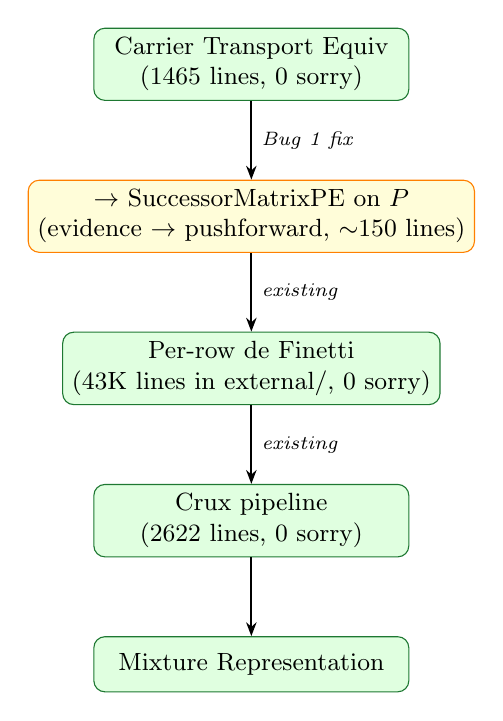
\begin{tikzpicture}[
  node distance=1.0cm and 2.5cm,
  box/.style={draw, rounded corners, minimum width=4cm,
    minimum height=0.7cm, align=center, font=\small},
  proved/.style={box, fill=green!12, draw=provedgreen},
  needed/.style={box, fill=yellow!15, draw=orange},
  gap/.style={box, fill=red!10, draw=gapred, dashed},
  arr/.style={-{Stealth[length=5pt]}, thick}
]
\node[proved] (carrier) {Carrier Transport Equiv\\(1465 lines, 0 sorry)};
\node[needed, below=of carrier] (pe) {$\to$ SuccessorMatrixPE on $P$\\(evidence $\to$ pushforward, $\sim$150 lines)};
\node[proved, below=of pe] (rowdf) {Per-row de Finetti\\(43K lines in external/, 0 sorry)};
\node[proved, below=of rowdf] (crux) {Crux pipeline\\(2622 lines, 0 sorry)};
\node[proved, below=of crux] (repr) {Mixture Representation};

\draw[arr] (carrier) -- node[right, font=\scriptsize\itshape] {Bug 1 fix} (pe);
\draw[arr] (pe) -- node[right, font=\scriptsize\itshape] {existing} (rowdf);
\draw[arr] (rowdf) -- node[right, font=\scriptsize\itshape] {existing} (crux);
\draw[arr] (crux) -- (repr);
\end{tikzpicture}
\end{center}

The key insight: if Bug~1 is fixed (carrier transport $\to$
successor-matrix PE), then the existing infrastructure---the
i.i.d.\ de Finetti theorem already formalized in 43{,}000 lines
of Lean---provides the row kernel construction automatically.
The cross-row coherence step and the cylinder mixing identity
then follow from the Crux file's proved conditional chain.

\paragraph{What the new bridge must prove.}
The bridge from carrier transport to \lean{SuccessorMatrixPartialExchangeable}
requires:

\begin{enumerate}[leftmargin=2em]
\item \textbf{Adjacent $\to$ general composition} ($\sim$30 lines):
  Compose \lean{carrierTransportEquivAdjacent} via \lean{Equiv.trans}
  and Nat induction on $|n - n'|$ to obtain the general $n \to n'$
  carrier Equiv.

\item \textbf{Evidence preservation $\to$ cylinder equality} ($\sim$50 lines):
  From the evidence-preserving Equiv on finite carriers, derive
  $P(\mathrm{cylinder}(xs)) = P(\mathrm{cylinder}(ys))$ whenever
  $\mathrm{evidenceOf}(xs) = \mathrm{evidenceOf}(ys)$, using the
  extension property $\mu(xs) = P(\mathrm{cylinder}(xs))$ and
  Markov exchangeability.

\item \textbf{Cylinder equality $\to$ pushforward equality} ($\sim$70 lines):
  From cylinder-level equality, derive the measure-level equality
  $\mathrm{Measure.map}(f \circ \sigma)(P) = \mathrm{Measure.map}(f)(P)$
  using the $\pi$-$\lambda$ theorem (Mathlib's
  \lean{MeasureTheory.ext\_of\_generate\_finite}).
\end{enumerate}

\subsection{Remaining mathematical gap: the wiring step}
\label{sec:wiring}

Even with the corrected strategy, a nontrivial wiring step remains:
connecting the \lean{SuccessorMatrixPartialExchangeable} property
to the existing infrastructure that builds
\lean{BuiltRowKernelOnExtension}.

The existing code path (Crux line 1066) extracts per-row
conditionally-IID row kernels from PE, but produces them with
\emph{unrestricted} row-process factorization.  The internal
theorem requires \emph{start-restricted} factorization
(\lean{StartRestrictedRowKernelData}).  As noted in
\S\ref{sec:crossrow}, PE alone does not imply start-restricted
invariance---this is where the carrier transport contributes its
essential content.

The precise wiring is:
\begin{enumerate}[leftmargin=2em]
\item From PE, build unrestricted row kernels with
  \lean{hEval} and \lean{hPi} (existing, Crux line 1352).
\item From carrier transport (via the general $n \to n'$ Equiv),
  prove \lean{StartRestrictedRowSuccessorPermInvariant}
  (existing, Crux line 1591).
\item Upgrade the unrestricted row factorization to start-restricted
  factorization using the permutation invariance
  (this is the step that needs explicit proof, $\sim$200 lines).
\item From start-restricted factorization + per-row conditional IID,
  derive \lean{CrossRowCoherenceStep} (the induction step).
\item Apply the induction combinator (existing, Crux line 695)
  to obtain \lean{CrossAnchorProductIdentity}, then
  \lean{CylinderMixingIdentity\_P} and the full representation.
\end{enumerate}

Step~(3) is the key mathematical step: showing that permutation
invariance of 1D marginals, combined with per-row conditional IID
from de Finetti, gives the start-restricted factorization.
Step~(4) follows from step~(3) by the trajectory structure:
conditioned on the full trajectory $\omega$, the
transition from state $a$ to the next state uses row-$a$'s kernel,
and the continuation from the next state is determined by the
remaining row kernels, which are conditionally independent given $\omega$.

\subsection{Summary of recommended steps}

\begin{center}
\small
\begin{tabular}{clcc}
\hline
\textbf{Priority} & \textbf{Step} & \textbf{Est.\ lines} & \textbf{Dependencies} \\
\hline
1 & Adjacent $\to$ general Equiv composition & 30 & Carrier transport \\
2 & Evidence preservation $\to$ \lean{SuccessorMatrixPE} & 150 & Step 1 \\
3 & Start-restricted upgrade from PE + carrier transport & 200 & Step 2, Crux \\
4 & \lean{CrossRowCoherenceStep} from conditional IID & 100 & Step 3, de Finetti \\
5 & Instantiate \lean{BuildRowKernelOnRecurrentExtension} & 50 & Steps 2--4 \\
\hline
& \textbf{Total estimated new code} & \textbf{$\sim$530} & \\
\hline
\end{tabular}
\end{center}

Step~2 is the most architecturally important: it connects the proved
carrier transport (1465 lines) to the proved de Finetti infrastructure
(43{,}000 lines) through the proved Crux pipeline (2622 lines).  Once
this bridge exists, the remaining steps are consequences of existing
proved chains.

The Euler trail archive (1225 lines, 0 sorry) provides an alternative
to Steps~1--2: the CopyPerm group gives the joint finite-dimensional
invariance more directly than composing adjacent transpositions.
Integrating this archive into the active framework would require
adapting from the \lean{EulerGraph}/\lean{edgeTok} data model to the
\lean{rowVisitCylinderEventUpToPrefixCarrier} framework, estimated at
$\sim$200 lines.

%% ========================================================================
\section{The Broader Context}
\label{sec:context}
%% ========================================================================

\subsection{Classical de Finetti (i.i.d.\ case)}

The i.i.d.\ case of de Finetti's theorem is \emph{fully formalized} in
the companion project \texttt{Mettapedia/external/exchangeability/}
(${\sim}43{,}000$ lines of Lean, zero \texttt{sorry}).  Three independent
proofs are provided:

\begin{enumerate}[leftmargin=2em]
\item \textbf{Via reverse martingale convergence} (default; follows
  Kallenberg 2005).
\item \textbf{Via $L^2$ bounds} (lightest dependencies; elementary).
\item \textbf{Via the mean ergodic theorem} (deepest theory; connects to
  dynamical systems).
\end{enumerate}

The main theorem proved is:
\[
\text{Contractable} \;\Longleftrightarrow\;
\text{Exchangeable} \;\Longleftrightarrow\;
\text{Conditionally i.i.d.}
\]
for infinite sequences on standard Borel spaces.

\subsection{Solomonoff bridge: exchangeability implies count sufficiency}

The file \lean{SolomonoffExchangeable.lean} proves the analogous
count-sufficiency result for the i.i.d.\ (binary) case at the
\emph{semimeasure} level---directly connecting to Solomonoff's
universal prior:

\begin{lstlisting}
-- From SolomonoffExchangeable.lean (binary/i.i.d. case):
theorem semimeasureExchangeable_same_counts
    {μ : BinString → ℝ}
    (hexch : SemimeasureExchangeable μ)
    {n : ℕ} (xs₁ xs₂ : Fin n → Bool)
    (hcount : countTrue xs₁ = countTrue xs₂) :
    μ (List.ofFn xs₁) = μ (List.ofFn xs₂)
\end{lstlisting}

Under exchangeability, the Solomonoff-style predictor depends only on
counts, not on ordering.  This is the binary analogue of the Markov
count-sufficiency result in Section~\ref{sec:proved}: the Markov version
replaces \lean{countTrue} (a single count) with \lean{transCount}
(a $k \times k$ matrix of transition counts).

This justifies the ``evidence is what you carry'' design of PLN:
under exchangeability, binary evidence counts $(n^+, n^-)$ are
sufficient statistics for prediction.

\subsection{The complete chain (with gap)}

The intended end-to-end chain is:

\begin{center}
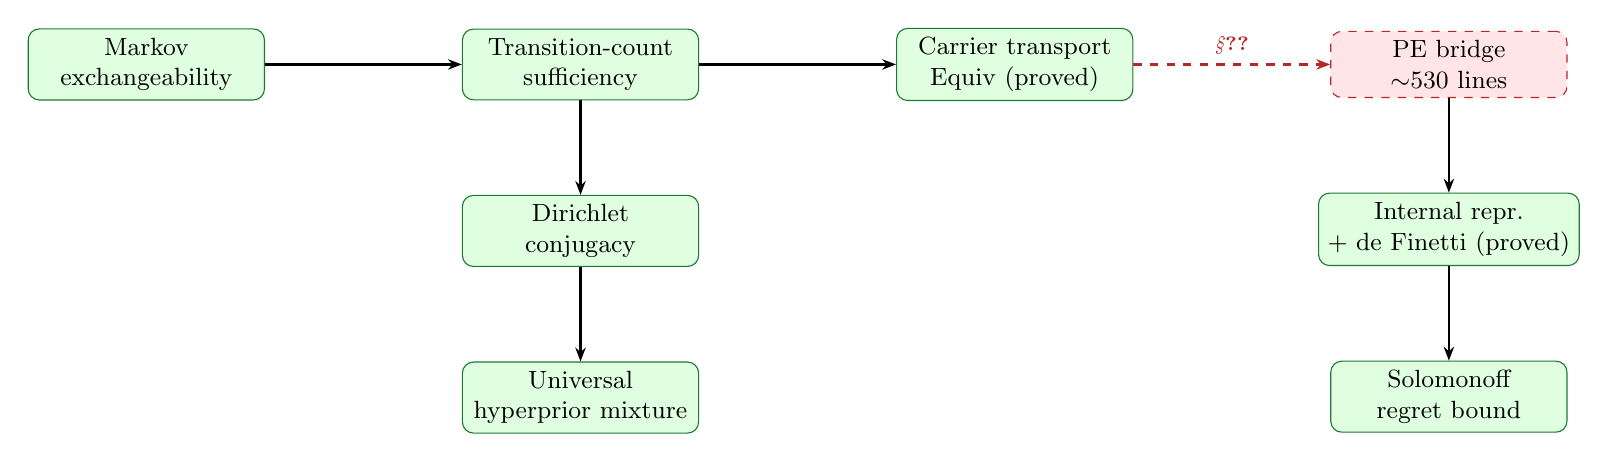
\begin{tikzpicture}[
  node distance=1.2cm and 2.5cm,
  box/.style={draw, rounded corners, minimum width=3cm,
    minimum height=0.8cm, align=center, font=\small},
  proved/.style={box, fill=green!12, draw=provedgreen},
  gap/.style={box, fill=red!10, draw=gapred, dashed},
  arr/.style={-{Stealth[length=5pt]}, thick}
]
\node[proved] (exch) {Markov\\exchangeability};
\node[proved, right=of exch] (counts) {Transition-count\\sufficiency};
\node[proved, below=of counts] (dirichlet) {Dirichlet\\conjugacy};
\node[proved, below=of dirichlet] (hyperprior) {Universal\\hyperprior mixture};
\node[proved, right=2.5cm of counts] (carrier) {Carrier transport\\Equiv (proved)};
\node[gap, right=of carrier] (bridge) {PE bridge\\$\sim$530 lines};
\node[proved, below=of bridge] (internal) {Internal repr.\\+ de Finetti (proved)};
\node[proved, below=of internal] (solomonoff) {Solomonoff\\regret bound};

\draw[arr] (exch) -- (counts);
\draw[arr] (counts) -- (dirichlet);
\draw[arr] (dirichlet) -- (hyperprior);
\draw[arr] (counts) -- (carrier);
\draw[arr, dashed, gapred] (carrier) -- node[above, font=\scriptsize\itshape]
  {\S\ref{sec:strategy}} (bridge);
\draw[arr] (bridge) -- (internal);
\draw[arr] (internal) -- (solomonoff);
\end{tikzpicture}
\end{center}

With carrier transport proved and the structural audit complete
(\S\ref{sec:strategy}), closing the remaining bridge ($\sim$530 lines)
from evidence preservation to successor-matrix partial exchangeability
would complete the chain from Markov exchangeability to a mixture
representation with Solomonoff-style dominance guarantees.

%% ========================================================================
\section{File Inventory}
\label{sec:inventory}
%% ========================================================================

All files are in the \texttt{Mettapedia} Lean project, available at\\
\url{https://github.com/zariuq/ai-agents/tree/main/lean-projects/mettapedia/Mettapedia/Logic/}.

\begin{center}
\small
\begin{tabular}{llrl}
\hline
\textbf{Layer} & \textbf{File} & \textbf{Lines} & \textbf{Status} \\
\hline
Definitions & \texttt{MarkovExchangeability.lean} & 146 & {\color{provedgreen}0 sorry} \\
Conjugacy & \texttt{EvidenceDirichlet.lean} & 496 & {\color{provedgreen}0 sorry} \\
Predictor & \texttt{MarkovDirichletPredictor.lean} & 497 & {\color{provedgreen}0 sorry} \\
Hyperprior & \texttt{MarkovDirichletHyperpriorMixture.lean} & $\sim$50K & {\color{provedgreen}0 sorry} \\
Domain bridge & \texttt{MarkovExchangeabilityBridge.lean} & 600+ & {\color{provedgreen}0 sorry} \\
Solomonoff & \texttt{SolomonoffExchangeable.lean} & 200+ & {\color{provedgreen}0 sorry} \\
Recurrence & \texttt{MarkovDeFinettiRecurrence.lean} & --- & {\color{provedgreen}0 sorry} \\
Hard core & \texttt{MarkovDeFinettiFortiniBridgeCore.lean} & 1843 & {\color{provedgreen}0 sorry} \\
Hard crux & \texttt{MarkovDeFinettiFortiniBridgeCrux.lean} & $\sim$2600 & {\color{provedgreen}0 sorry} \\
Carrier core & \texttt{MarkovDeFinettiCarrierTransportCore.lean} & 319 & {\color{provedgreen}0 sorry} \\
Carrier bridge & \texttt{MarkovDeFinettiCarrierTransport.lean} & 1146 & {\color{provedgreen}0 sorry} \\
Surface & \texttt{MarkovDeFinettiFortiniBridgeCanonical.lean} & 131 & {\color{provedgreen}0 sorry} \\
\hline
De Finetti & \texttt{external/exchangeability/} & 43K & {\color{provedgreen}0 sorry} \\
\hline
\end{tabular}
\end{center}

\paragraph{Note on ``0 sorry.''}
Every file listed above compiles without \texttt{sorry}.  However, the
canonical surface file (\texttt{...Canonical.lean}) proves the
representation theorem \emph{only under bridge assumptions}
stated as hypotheses (see \S\ref{sec:bug2}).  The core mathematical
content---constructing the row kernel from exchangeability---is
encoded as three \lean{def \ldots\ : Prop} declarations that are
used as hypotheses but never instantiated.  The gap manifests as
uninstantiated assumptions, not as incomplete proofs.

%% ========================================================================
\section*{References}
%% ========================================================================

\begin{enumerate}[leftmargin=2em, label={[\arabic*]}]

\item P.~Diaconis and D.~Freedman, ``De Finetti's theorem for Markov
  chains,'' \emph{Ann.\ Probab.}, vol.~8, no.~1, pp.~115--130, 1980.

\item S.~Fortini, L.~Ladelli, and E.~Regazzini, ``Exchangeability,
  predictive distributions and parametric models,''
  \emph{Sankhy\=a A}, vol.~62, pp.~86--109, 2000.

\item T.~Sato, ``A statistical learning method for logic programs with
  distribution semantics,'' in \emph{Proc.\ 12th Int.\ Conf.\ Logic
  Programming (ICLP)}, 1995.

\item M.~Hutter, \emph{Universal Artificial Intelligence: Sequential
  Decisions Based on Algorithmic Probability}, Springer, 2005.

\item R.~J.~Solomonoff, ``A formal theory of inductive inference,''
  \emph{Inform.\ Control}, vol.~7, pp.~1--22, 224--254, 1964.

\item O.~Kallenberg, \emph{Probabilistic Symmetries and Invariance
  Principles}, Springer, 2005.

\item B.~de~Finetti, ``La pr\'evision: ses lois logiques, ses sources
  subjectives,'' \emph{Ann.\ Inst.\ H.\ Poincar\'e}, vol.~7,
  pp.~1--68, 1937.

\end{enumerate}

\end{document}
